\documentclass[12pt]{article}
\usepackage[left=12mm,top=0.5in,bottom=5in]{geometry}
\usepackage[utf8]{inputenc} 
\usepackage[T2A]{fontenc} 
\usepackage{enumitem} 
\usepackage{graphicx} %зураг
\usepackage[mongolian]{babel}

\usepackage{anysize}
\marginsize{3cm}{1.5cm}{2cm}{2cm}     

\begin{document}
	
	
	
\section     {Гарчиг}

\section     {Төслийн хэсэг}
               0.1  Оршил………………………………………………………………………………                ..1                           
               
               1.1  Хэрэглэгчийн тухай мэдээлэл ……………………………………………………………………………………                   
               ..2
               
               1.2  Хэрэглэгчийн үйл ажиллагааны онцлог …………………………………………………………………………………………         
               ..5
               
               1.3  Хэрэглэсэн нэр томъёоны тодорхойлолт …………………………………………………………………………                       ..7
               
               1.4  Лавлах материал…………………………………………………………………………          ..8
               
               1.5  Хэрэглэгчийн функциональ шаардлага …………………………………………………………………………………                    ..11
               
               1.6  Хэрэглэгчийн функциональ бус шаардлага                                          ..10
               
               
\section     {II бүлэг.}  Системийн шинжилгээ

               1.   Buseniss process diagram ………………………………………………………………………………………………………               
                ..27
               
               2.	Activity diagram ………………………………………………………………………………………………………                   
                ..33
               
               3.	Class diagram ………………………………………………………………………………………………………                   
                ..37
                
               4.   Use case diagram
               ………………………………………………………………………………………………………                 
                ..40
                
               5.   Sequnence diagram
               ………………………………………………………………………………………………………                   
                ..37
                
               6.   Workflow diagram
               ………………………………………………………………………………………………………                  
                ..37
                
               7.   ERD diagram
               ………………………………………………………………………………………………………                  
                ..37
                
               8. Statechart diagram
               ………………………………………………………………………………………………………                  
               ..38
               
                
                
               
\section     {III бүлэг.} Ижил төстэй програмийн судалгаа

               1.   Үүрэг зориулалт…………………………………………………………………………………………………  
               
               2.   Зорилго зорилт……………………………………………………………………………………………………
                   
               
\section     {IV Бүлэг.} 
    
               3.	Ерөнхий дүгнэлт
               
               4.	Ашигласан материалууд    
        
                 



	
	\section                            {ОРШИЛ}
	
	Сүүлийн үед мэдээллийн технологи асар хурдацтай хөгжиж байгаагаас байгууллгага, аж ахуйн нэгжийн үйл ажиллагааны хэв маяг ч өөрчлөгдөж байна. 
	Ийнхүү албан байгууллага, хувь хүн, үйлдвэрүүдийн үйл ажиллагаа компьютер буюу тооцоолон бодох машинтай салшгүй холбоотой болсон ба тэр дундаа хүний хийх ажлыг хөнгөвчлөх, ажлын бүтээмжийг өндөрсгөх зэрэг асуудал нь нэн чухлаар тавигдаж байгаа. 
	Өнөөгийн мэдээллийн зуун гэж нэрлэгдсэн энэ үед хэн мэдээлэл сайн олж чадаж байна тэр чинээгээрээ амжилт олж чадах болсон. Иймд аливаа байгууллагын үйл ажиллагааг зохион байгуулах, мэдээллийн урсгалыг тодорхой болгож, мэдээллийг хурдан дамжуулах шаардлага зайлшгүй тулгар ч байна. Иймд интернет болон компьютерийн тусламжтай Сургуулийн цахим хуудсийг ажиллуулах нь багш оюутнууд ажил хичээлээ явуулхад тулгарсан ямар нэг асуудлийг шийдхэд нэн чухал үүрэг гүйцэтгэх юм.
	Ижил төстэй програмын судалгаа
	Энэ хүү санал асуулгийн модул нь Facebook-ийн Poll гэх модулаас санаа авсан бөгөөд хувь хүний хоорондийн групп чат болон хуудасны үйл ажиллагааны талаарх хуудасны нийт бүх гишүүдээс санал авах санал хураах үүднээс ашигладаг.Тухайн гишүүдэд санал асуулгын талаарх дүн харагдах байдал нь өнгө болон  хувиар илэрхийлэгдэж харагдах ба хэрэглэгчид энгийн бөгөөд ойлгомжтой ашиглахад хялбар байна. 
	
	
	
	\section     {Зорилго зорилт}
	
	Энэ модулын зорилго нь цахим сургуулийн орчинд ямар нэгэн хэлэлцэх чувхал асуудлийг шийдвэрлэх олон нийтийн санал хүсэлтийг түргэн шуурхай гаргах дэмжиж буй зүйл дэмжихгүй байгааг өнгө дүрсээр харуулах 
	зорилготой.
	
	
	
	
	\section  {Хэрэглэгчийн тухай мэдээлэл}
	
	Энэхүү модулийн хэрэглэгчид нь тухайн сургуулийн багш болон туслах багш бас оюутан юм. Хэрэглэгч нь ямар нэг үйл ажиллагаа болон тухайн системд байгаа гишүүдийн талаарх өөрсдийн санал хүсэлт болон санал асуулгийг авах зорилгоор чат болон тухайн хуудас хэрэглэгч өөрийн хуудсанд үүсгэж ашиглаж болно.
	
	\section  {Хэрэглэгчийн үйл ажиллагааны онцлог}
	
	{Админ:} Админ нь уг системын хэрэглэгч бөгөөд ямар нэгэн үйл ажиллагааны талаарх мэдээллийг оруулж өгснөөр гишүүдийн хооронд санал асуулга явуулах зорилгоор энэ модулыг ашгилна.
	
	
	{Багш:} Энэ модулыг  өөрийн хуудсанд үүсгэж оюутнуудийн санал бодлийг сонсох хичээлийн талаарх санал хүсэлт судалгаа хийх зорилгоор ашиглаж болно. 
	
	{Оюутан:} Энэ модулыг мөн өөрийн хувийн чат болон сургуулийн групп чатанд санал хүсэлтээр хэлэлцүүлэг хийх болон бөөнөөр шийдвэрлэх асуудлийг  явуулж болно.
	
	\title{Сургуулийн онлайн системийн санал асуулга модул}
	
	\author{О.Сугараа}
	
	\section{Хэрэглэгчийн функциональ шаардлага}
	\textit {Админ}
	\begin{itemize}
		[label=*, nosep]
        \item Нэвтрэх
		\item Мэдээллийг шинэчлэх 
		\item Санал асуулга үүсгэх
		\item Санал асуулга цэсыг сонгох
		\item Санал асуулга өгөх
		\item Санал асуулга харах
	\end{itemize}

	\textit {Хэрэглэгч}
	\begin{itemize}
		[label=*, nosep]
		\item Нэвтэрсэн байх
		\item Санал асуулга сонгох
		\item Санал асуулга өгөх 
		\item Санал асуулга харах
	\end{itemize}	
	
	
	\section{Хэрэглэгчийн функциональ бус шаардлага}
	\begin{center}
	\begin{itemize}
		[label=*, nosep]
		\item Санал асуулга өгсөн байх 
		\item Нэг хэрэглэгч нэг саналыг нэг л бөглөх
    \end{itemize}
	\end{center}
    






	
	\begin{figure}  \section       {II бүлэг.}  
		
		         Системийн шинжилгээ
		
		1.     Buseniss process diagram
		
		
		\centering
	   	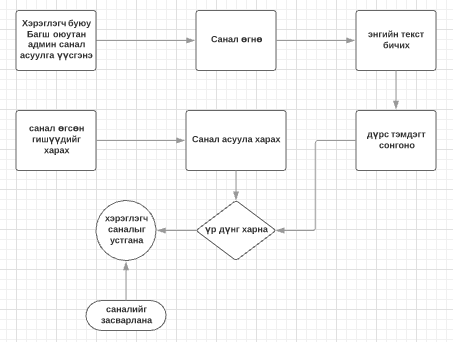
\includegraphics[width=0.7\linewidth]{./p}
		\caption{}
		\label{fig:p}
			\end{figure}
		
	\begin{figure}  \section       {II бүлэг.}  
			
		
		2.      Activity diagram	
		
			
			\centering
			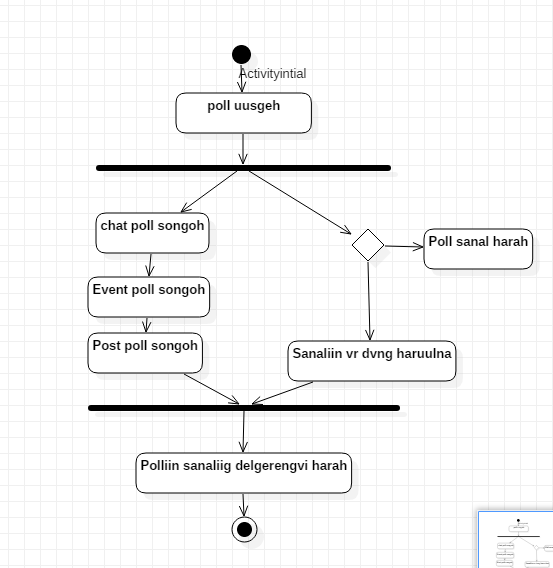
\includegraphics[width=0.7\linewidth]{./a}
			\caption{}
			\label{fig:a}
		\end{figure}
	
	\begin{figure}  \section       {II бүлэг.}  
	
	
	    3.       Sequence diagram	
	
	
        	\centering
	        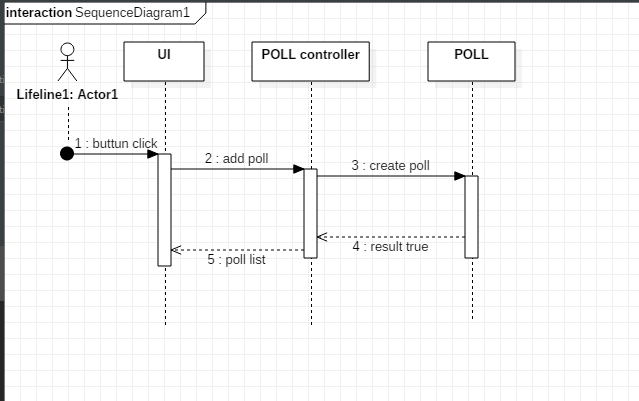
\includegraphics[width=0.7\linewidth]{./Sequ}
         	\caption{}
        	\label{fig:Sequ}
      \end{figure}

	    
	     4.      Use case diagram	
	    
   \begin{figure}
	    \centering
	    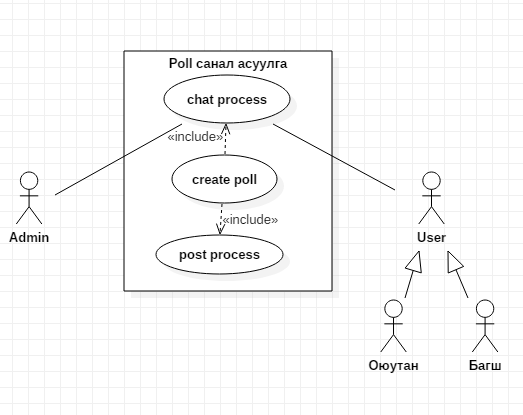
\includegraphics[width=0.7\linewidth]{./U}
	    \caption{}
	    \label{fig:U}
    \end{figure}

         5.       Class diagram
         
	 \begin{figure}
		\centering
		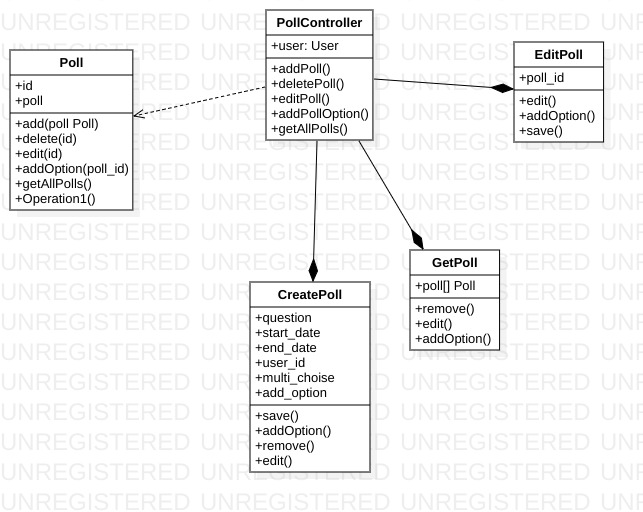
\includegraphics[width=0.7\linewidth]{./Main}
		\caption{}
		\label{fig:Main}
	\end{figure}


         6.      Дэлгэцийн зохиомж         

     \begin{figure}
	    \centering
	    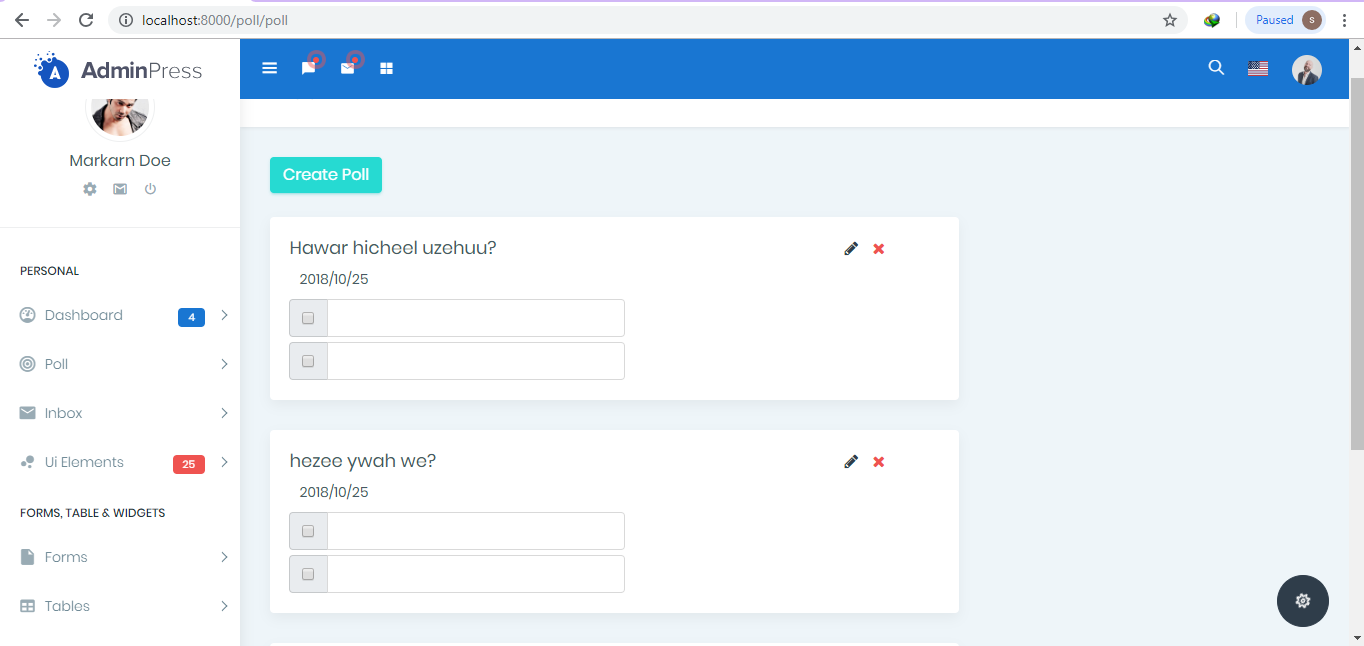
\includegraphics[width=0.7\linewidth]{./DE}
	    \caption{}
	    \label{fig:DE}
     \end{figure}
 
         7. Төлвийн диаграм

     \begin{figure}
    	\centering
	    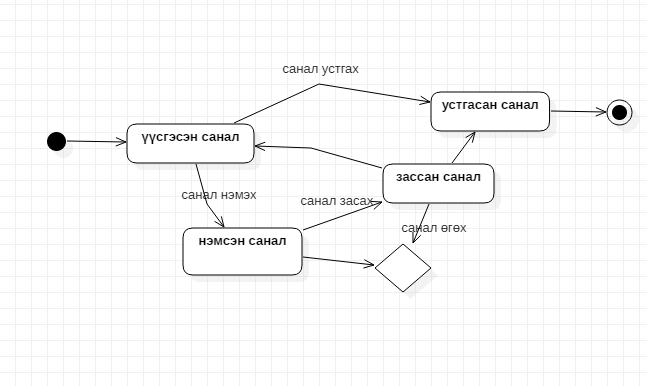
\includegraphics[width=0.7\linewidth]{./Tolowo}
	    \caption{}
	    \label{fig:Tolowo}
     \end{figure}


	
	\section     {III бүлэг.} Ижил төстэй програмийн судалгаа
	
	\section	 {Үүрэг зориулалт}
	
	Анх 2001 оны 2 сарын 4 нд Марк Цукерберг Facebook-ийг Харвардын Их Сургуульд сурдаг хажуу өрөөнийхөө компьютерийн чиглэлээр суралцдаг хоёр найзтайгаа санаачлан хийж байв. Найзуудтайгаа байнга холбоотой байж болохуйц гүүр маягийн вэб сайтыг тэд анх бүтээхээр зорьж байв. Тийм ч учраас 2002 он хүртэл энэхүү сайт нь зөвхөн Харвард Коллежийн дотоод хүрээнд л ажиллаж байв. Ингээд 2002 оны 9 сараас хойш дэлхий дахинаа энэхүү том сүлжээ сайт нь нээгдэж байсан түүхтэй. Энэхүү том сүлжээ сайтийн нэгэн жижиг модул болох санал асуулга буюу (Poll)нь үүрэг зориулалтын хувьд хэрэглэгчийн хувийн чат болон групп чатанд бас ямар нэгэн үйл ажиллагаа явуулах зорилгоор хэрэглэгч үүсгэж ажиллуулах боломжтой бөгөөд үр дүнг тэр дор нь харуулах зориулалттай модул юм.Ямар нэгэн том жижиг асуудлийг олноор түргэн шуурхай шийдэх үр дүнг бий болгож чадна.  
	
	
	
	
	
	
	
	
	
		
	
	
	\section     {IV Бүлэг.} 
	
	\section     {Ерөнхий дүгнэлт}  
	
	
	Өнөөгийн мэдээллийн зуун гэж нэрлэгдсэн энэ үед хэн мэдээлэл сайн олж чадаж байна тэр чинээгээрээ амжилт олж чадах болсон. Иймд аливаа байгууллагын үйл ажиллагааг зохион байгуулах, мэдээллийн урсгалыг тодорхой болгож, мэдээллийг хурдан дамжуулах шаардлага зайлшгүй тулгар ч байна. Иймд интернет болон компьютерийн тусламжтай Сургуулийн цахим хуудсийг ажиллуулах нь багш оюутнууд ажил хичээлээ явуулхад тулгарсан ямар нэг асуудлийг шийдхэд нэн чухал үүрэг гүйцэтгэснээр хэрэглэгчийн цаг завийг хэмнэж түргэн шуурхай ажиллаж ямар нэгэн асуудлийг хурдан шуурхай шийдэх боломжийг олгож өгнө гэж ойлгож болох юм.
	
	
	
	\section     {Ашигласан материалууд}   
	
	
	1.www.Facebook.com   
	
	2.www.wikipedia  
	
\end{document}             

    
               
               
               
               
               
               
               
               

               
                 
               
               
               
               
               
               
               
               
               
               
               
               
               
               
               
               
               
               
               
               
               
               
               
               
               
               
               
               
               
               
               
               
               
               
               
               
               
               
               
               
               
               
               
 
